\chapter{Initial Investigation}

There exist three algorithms for computing the Nash Equilibria of a game:
Support Enumeration, Vertex Enumeration and Lemke Howson algorithm. Thus,
firstly an exploration into the properties and execution times was needed to
verify which algorithm would be the most appropriate. This investigation, along
with a description of each algorithm (in the two-player case), is detailed in the next few sections.

\section{Support Enumeration Algorithm}
For a non-degenerate two player game $$G = (2, (S_{i})_{i = 1, 2}, (u_{i})_{i =
1, 2})$$, the following algorithm yields all Nash equilibria:
    \begin{itemize}
        \item For all $1 \le k \le min(|S_{1}|, |S_{2}|)$,
        \item and each $I, J \subset S_{1}, S_{2}$, respectively, with $|I| =
        |J| = k$,
        \item solve $\sum_{i \in I}{\sigma_{i}b_{i, j} = v}$,
        $\sum_{j \in J}{a_{i, j}\sigma_{j} = v}$ for all $j \in J$, $i \in I$ respectively
        \item such that $\sum_{i \in I}{\sigma_{i}}=1$ and $\sum_{j \in
        J}{\sigma_{j}}=1$ with $\sigma_{i}, \sigma_{j} \ge 0$
        \item and the best response condition in section \ref{} is satisfied.
    \end{itemize}




\section{Vertex Enumeration Algorithm}


\section{Lemke Howson Algorithm}


\section{Execution Times}
The code used to obtain the results in this section can be found in Appendix ...

From figure \ref{}, it can be seen that until the Defector has five opponents,
each algorithm has approximately the same running time. 

\begin{figure}
    \begin{center}
        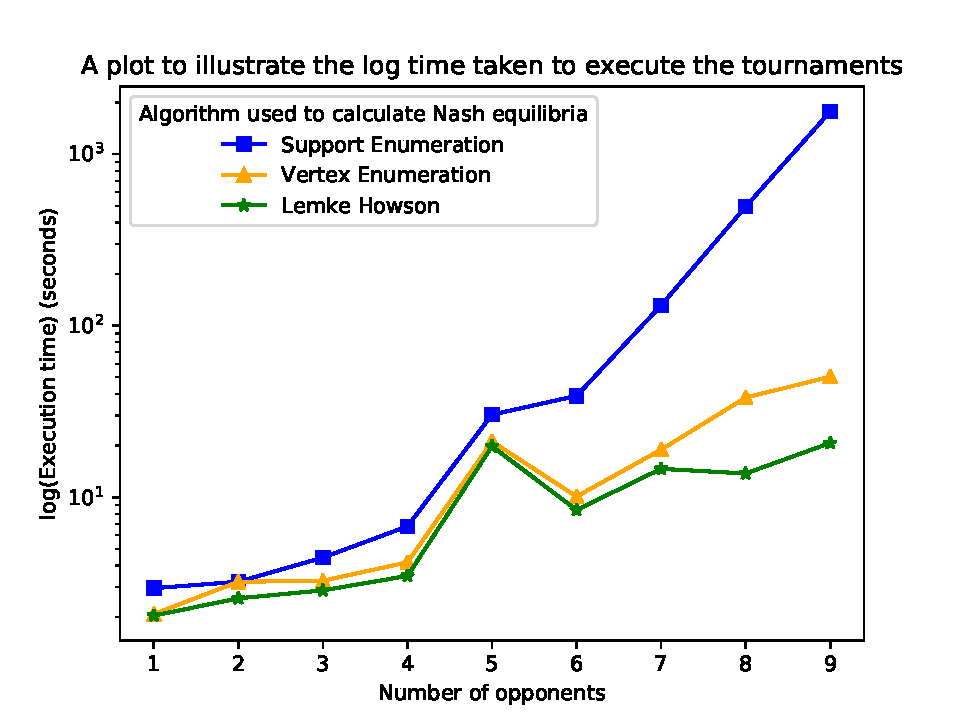
\includegraphics{log-timing-graph.pdf}\label{LogTimingGraph}
        \caption{A graph to show the results of the timed experiments for each of the three stated algorithms.}
    \end{center}
\end{figure}

After this, as the number of opponents increases it is clear that the support
enumeration algorithm blows up significantly quicker exponentially in 
comparison to boththe Vertex Enumeration and Lemke Howson algorithm. The latter 
two algorithms seem to have a similar execution time until the number of
opponents reaches eight and nine. This is when the Vertex Enumeration
algorithm's execution time starts to grow faster than the Lemke Howson algorithm.